\synctex=1
% Created 2014-12-01 Mon 10:14
\documentclass[bigger]{beamer}
%% \usepackage[utf8]{inputenc}
\usepackage[latin1]{inputenc}
\usepackage{times} %% o.w. fonts look like shit
\usepackage[T1]{fontenc}
\usepackage{graphicx}
\usepackage{float}

\usepackage{fixltx2e}
\usepackage{longtable}
\usepackage{wrapfig}
\usepackage{rotating}
\usepackage[normalem]{ulem}
\usepackage{amsmath}
\usepackage{textcomp}
\usepackage{marvosym}
%% \usepackage{wasysym}
\usepackage{amssymb}
\usepackage{hyperref}
\usepackage{url}


\usepackage[begintext=\textquotedblleft,endtext=\textquotedblright]{quoting}

\tolerance=1000
\usepackage{CSIC2}
\setbeamertemplate{navigation symbols}{}
\usetheme{default}

\newcommand{\blu}[1]{{\textcolor {blue} {#1}}}
\newcommand{\green}[1]{{\textcolor {green} {#1}}}


\newcommand{\Burl}[1]{\blu{\url{#1}}}


\author{Ramon Diaz-Uriarte}
% \date{}
\date{2021-09-21}
\title{Confidence intervals, p-values, and interpretation}
\hypersetup{
  pdfkeywords={},
  pdfsubject={},
  pdfcreator={Emacs 24.4.1 (Org mode 8.2.10)}}
\begin{document}

% \maketitle
% \begin{frame}{Outline}
% \tableofcontents
% \end{frame}


\begin{frame}
  \frametitle{I will draw some 95\% confidence intervals}

%%% There is a figure of this: CIexamples.pdf
  
%%%  


  %    this is the 0 line
  %    |	   
  % [------------*--------------] : results compatible with very relevant effects
  %                                most definitely this provides NO support for the null

  %       			 can have wide CI, but the fact that it includes 0 does not mean "the
  %   drug does not work". No statistical significance just means "not enough
  %   information"


				 
  %           [--*--]: the ideal thing

     

  % [-*-]  : like example below
  %   |
  %  [-*-] : all values are of little practical importance
  %          our results most compatible with no important effect
  %          (this ain't "the null is true"; it is "most likely little relevant")


    
  %                 |  
  %   [-------------*-------------]
  %   Anything could be happening: from very relevant positive to very relevant
  %   negative. Probably little can be said here.


  %   | [-*-] : significant but not relevant

  
  
  \ldots
\end{frame}


\begin{frame}
  \frametitle{Look at each of the figures}
  \begin{itemize}
  \item Which one(s) will be significant (at 0.05)?
  \item Which are compatible with strong positive effects?
  \item Which ones make it sensible to try to focus on this gene as a possible
    target?
    
    \begin{itemize}
    \item what if chasing this lead is extremely expensive or risky (side effects?)?
    \item what if it is cheap?
    \end{itemize}
  \item Which one(s) make it sensible to forget about this gene as a possible
    target?
  \item We are using 95\%. What if we used 99\%? Or 90\%?
  \end{itemize}
\end{frame}




\begin{frame}
   \centering
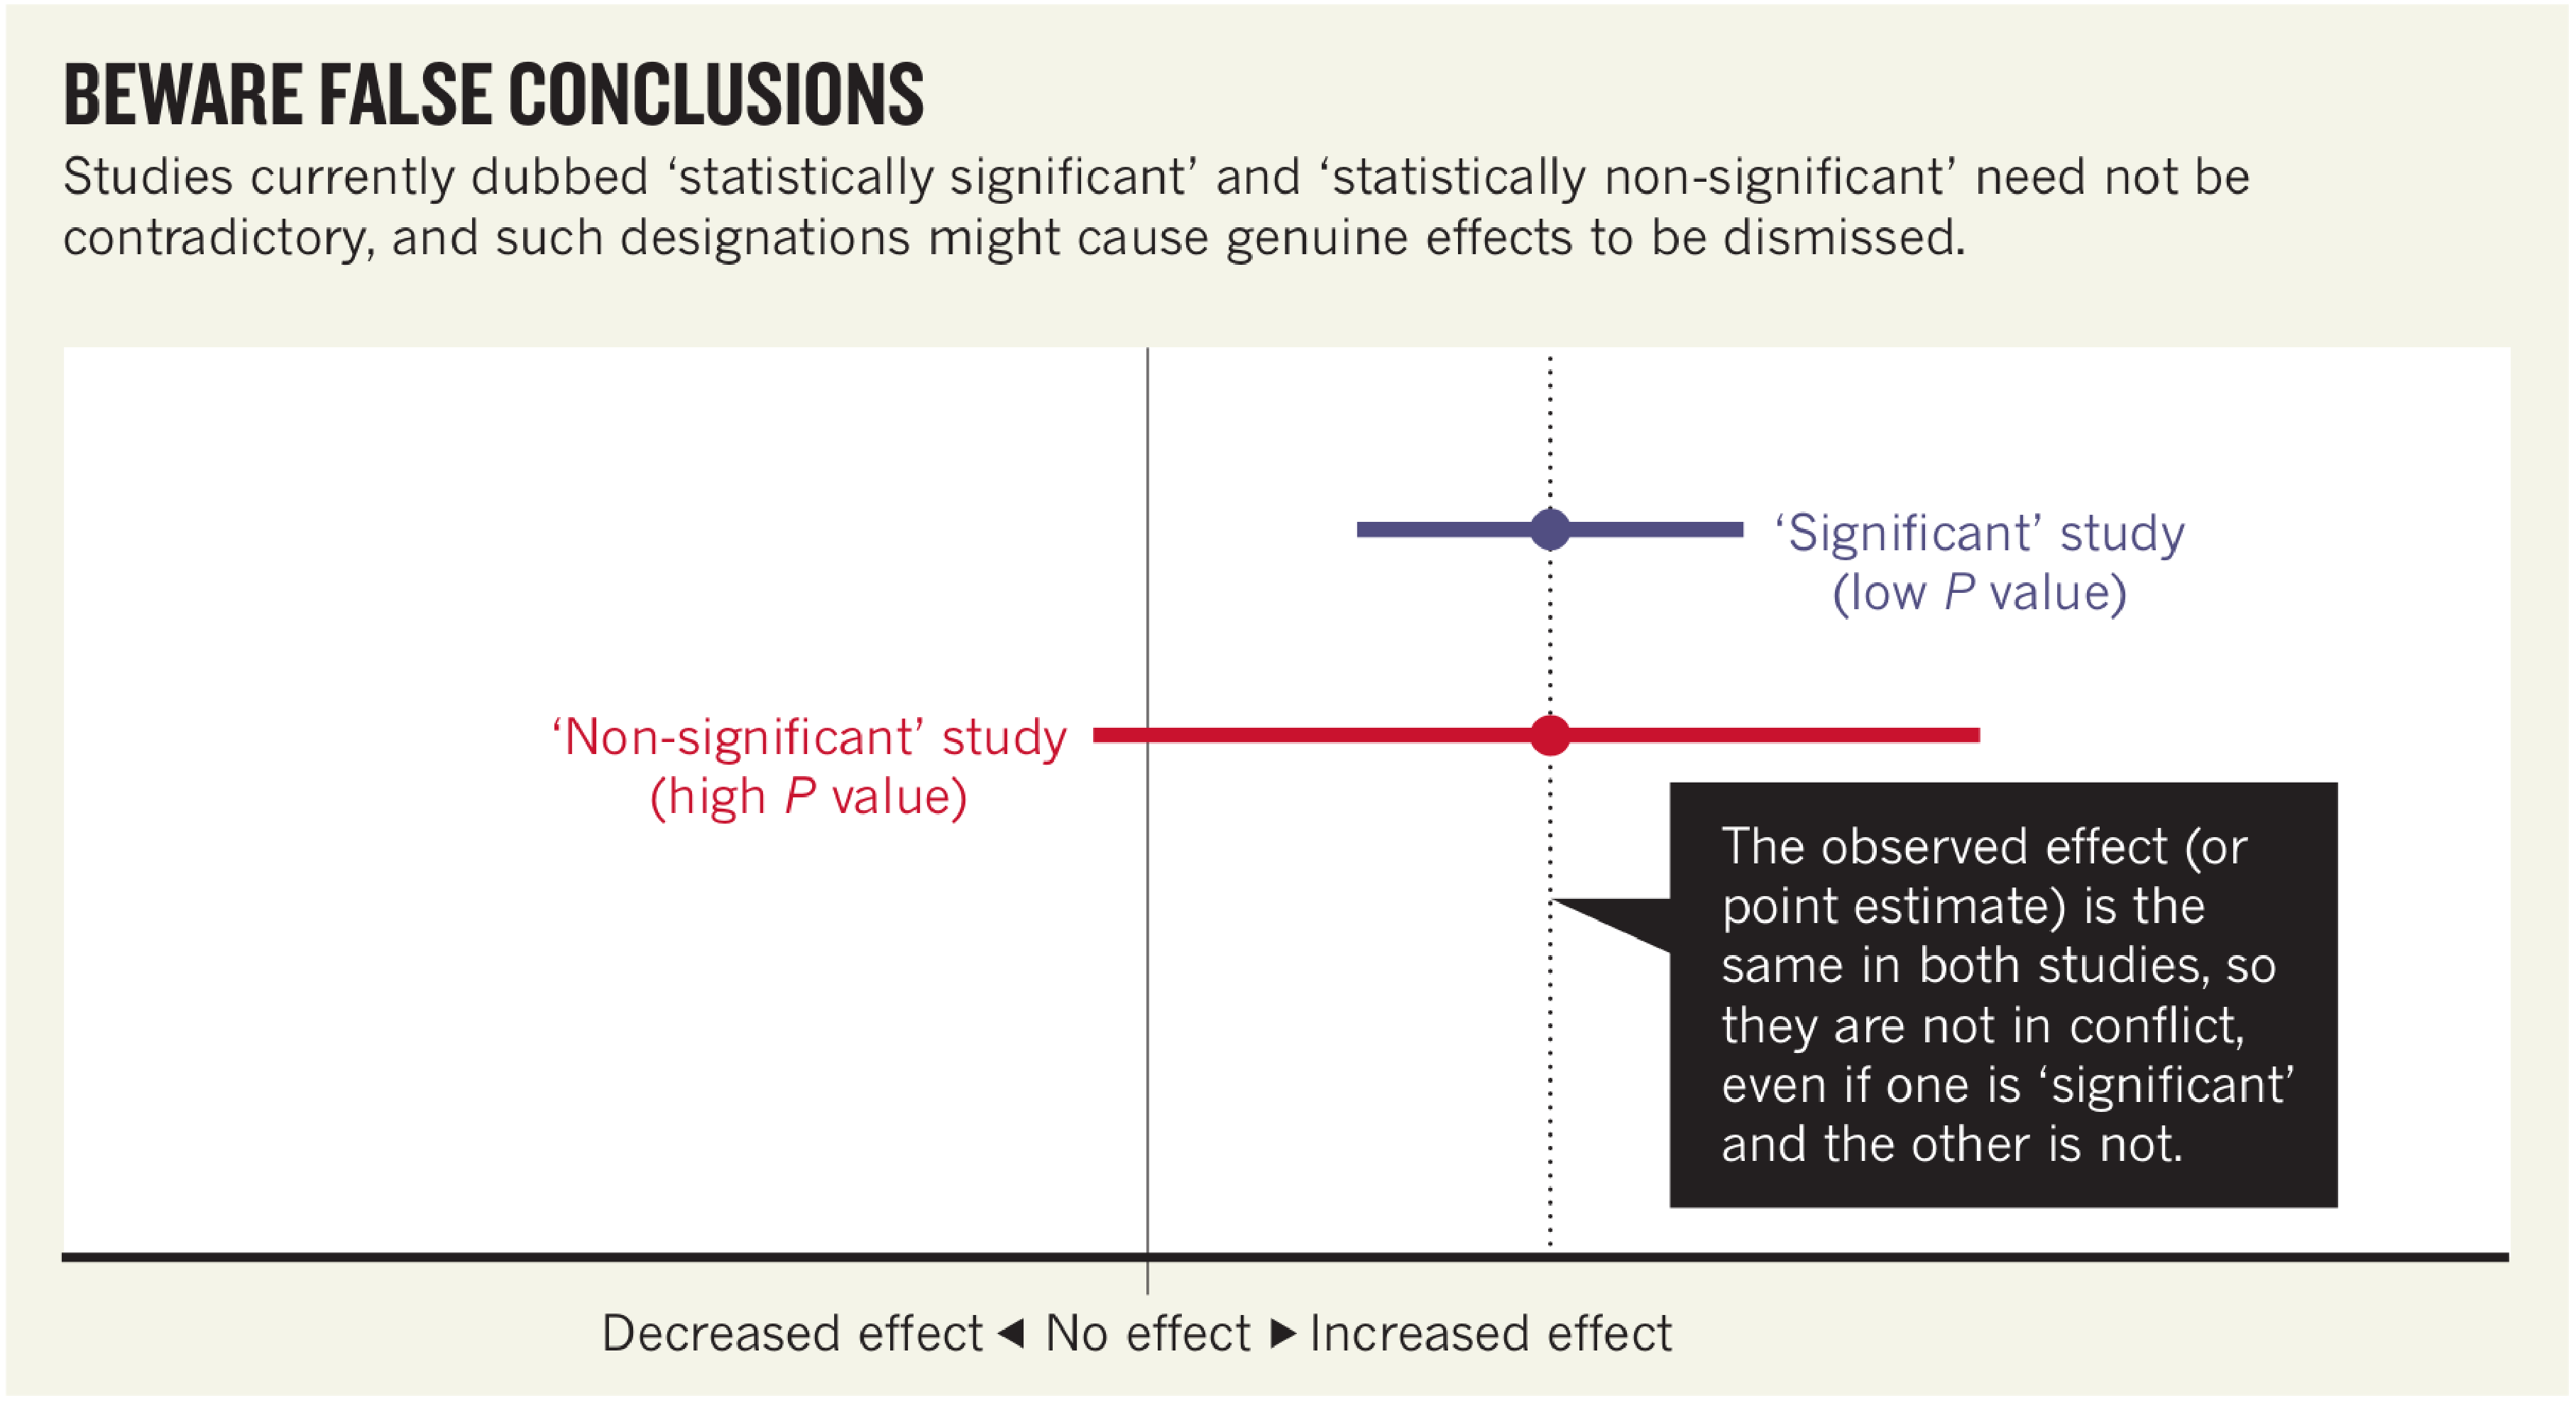
\includegraphics[width=11.5cm,keepaspectratio]{amrhein.pdf}

{\scriptsize From Amrhein et al., 2019. \textit{Retire statistical significance},
  Nature, 305.}
\end{frame}


\begin{frame}
\frametitle{Hypothesis vs.\ significance testing}

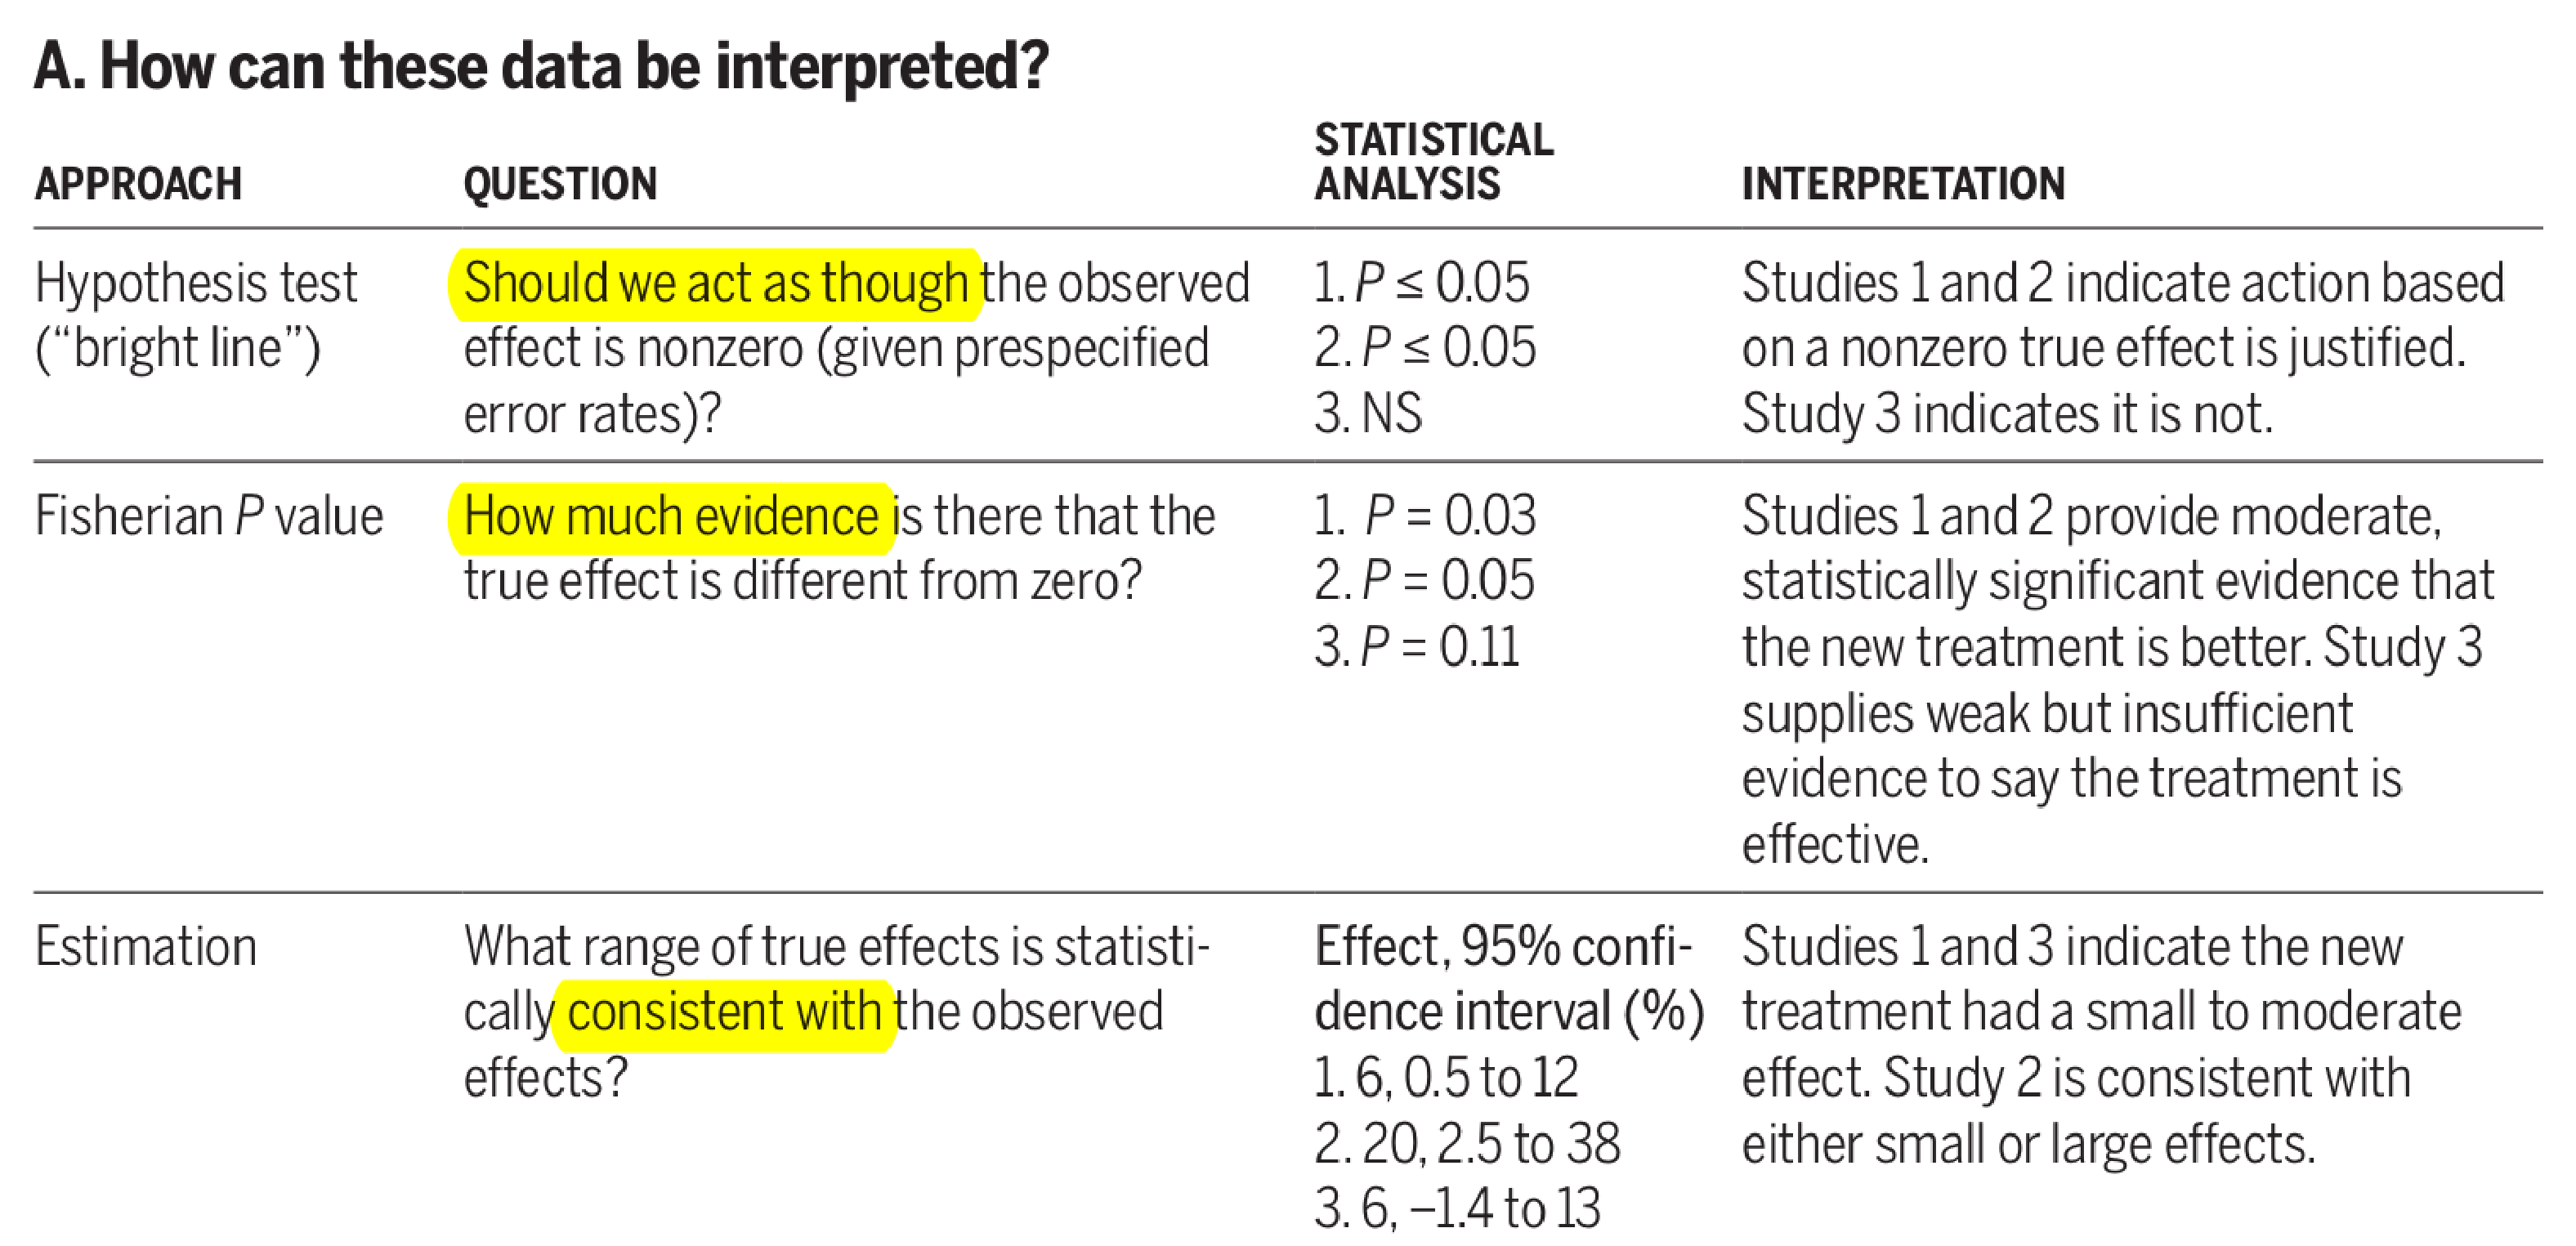
\includegraphics[width=11.5cm,keepaspectratio]{goodman.pdf}
  
{\scriptsize From Goodman, 2016, \textit{Aligning statistical and scientific
  reasoning}, Science, 352.}
\end{frame}




\begin{frame}
  \frametitle{A particular model, some assumptions}
  \begin{itemize}
  \item We are making assumptions
  \item There is an underlying model
  \item P-value, CI, constructed based upon the model and its assumptions.
  \end{itemize}
\end{frame}


\begin{frame}
  \frametitle{}
  \begin{itemize}
  \item Decision: include costs of mistakes (more later)
  \item What p-value? Depends on context. Sometimes we might want it much, much,
    much smaller.
  \end{itemize}
\end{frame}



\begin{frame}
  \frametitle{Context is key}

 \begin{quoting}
    Dichotomous conclusions can be useful for pinning down discoveries of
    gene variants for osteoporosis, new bosons or carcinogens, say.

    \vspace*{15pt}
    But focusing on effect sizes can often be better than determining
    whether an effect exists.
  \end{quoting}
  
  Ioannidis, letter to Nature, 28 March, 2019, vol.\ 567. ``Retiring significance: a
  free pass to bias''
  
\end{frame}



\begin{frame}
  \frametitle{Taking someone to trial and presumption of innocence analogy}
  \begin{description}
  \item[Significance and hypothesis testing] Is there enough evidence to sent this
    person to jail? How likely is, if she were innocent, that she committed
    the crime?
    \vspace*{15pt}
    
  \item[Estimate] But I really think she is guilty. Or ``but the evidence is most
    compatible with her being guilty (though we cannot show it beyond reasonable
    doubt)''.

    \vspace*{15pt}    
  \item[Bioquivalence] You have to show your innocence.

    \vspace*{15pt}    
  \end{description}
\end{frame}







\begin{frame}
  \frametitle{Let's go back to the initial cases}
  \ldots
  %% They should be in the blackboard. Same as in CIexamples.pdf
\end{frame}

%\section{Some references}


\begin{frame}
  \frametitle{Look at each of the figures}
  \begin{itemize}
  \item Which one(s) will be significant?
  \item Which are compatible with strong positive effects?
  \item Which ones make it sensible to try to focus on this gene as a possible
    target?
    \begin{itemize}
    \item what if chasing this lead is extremely expensive or risky (side effects?)?
    \item what if it is cheap?
    \end{itemize}
  \item Which one(s) make it sensible to forget about this gene as a possible
    target?
  \item We are using 95\%. What if we used 99\%? Or 90\%?
  \end{itemize}
\end{frame}




\begin{frame}
  \frametitle{Does all of this matter?}
  \begin{itemize}
  \item A lot!!
  \item And what about wide CIs?
  \item Many studies seriously misinterpreted. It has happened a lot, with
    serious consequences with the covid pandemic.
  \end{itemize}
\end{frame}


\begin{frame}
\frametitle{}

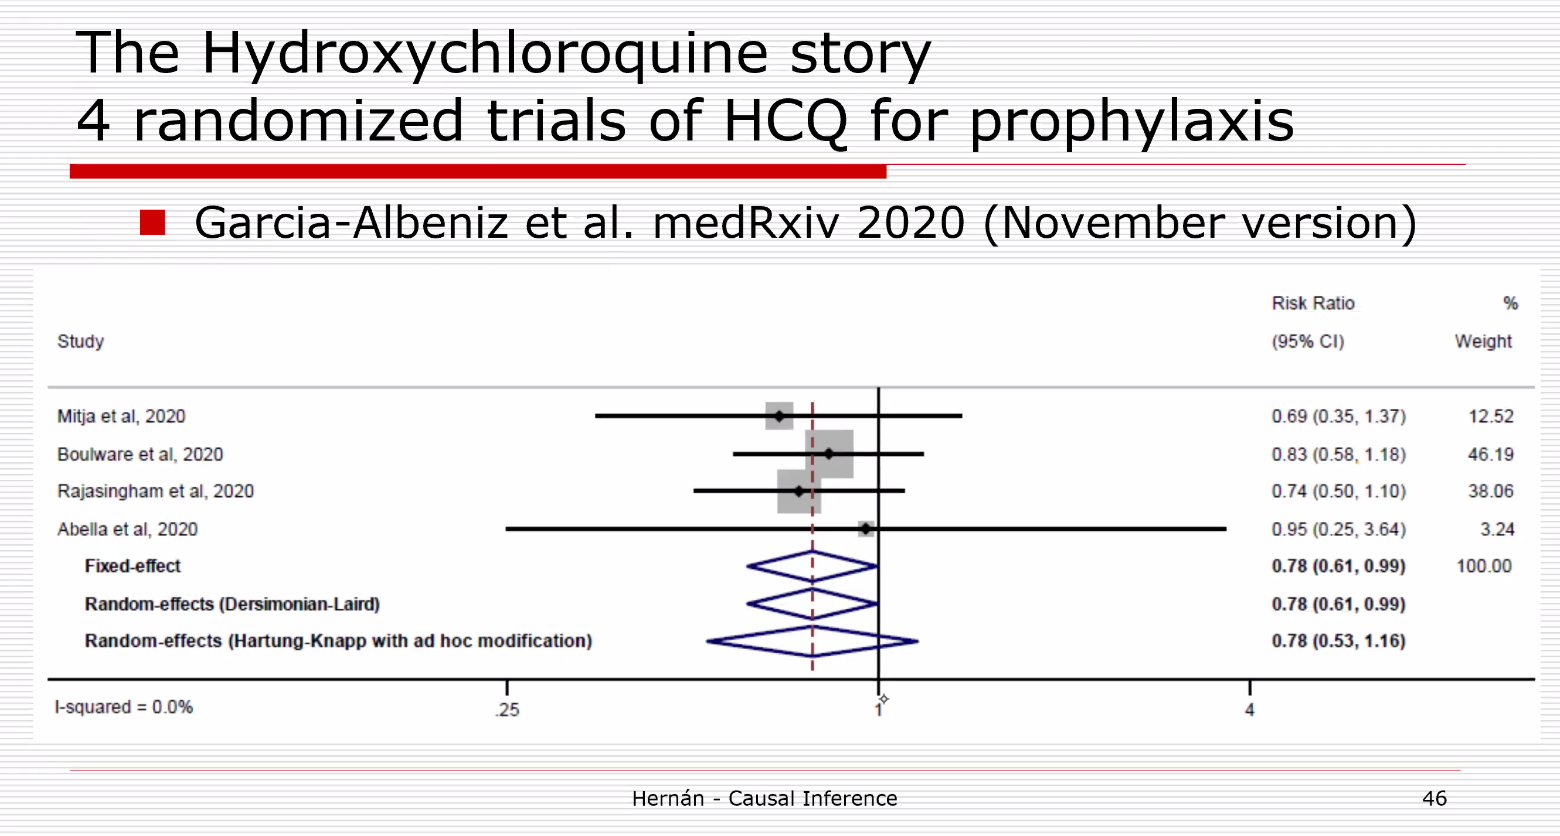
\includegraphics[width=11.5cm,keepaspectratio]{Hernan-6.png}
  
{\scriptsize From Miguel Hern�n's talk, Causal inference, ``Epidemiological
  Research Methods in the COVID-19 Pandemic'', IAP, 2021-06,14. Also Garc�a-Alb�niz et
al., 2021, \Burl{https://www.medrxiv.org/content/10.1101/2020.09.29.20203869v4.full}}
\end{frame}




\begin{frame}
  \frametitle{Wide CIs: problems and consequences of misinterpretations }
  \begin{itemize}
  \item Many papers published with huge CI are papers with no information, basically
  \item But then, that leads to people believe that the drug is not effective
  \item That makes further additional studies unlikely or impossible because "we
    already know it does not work" (which is the wrong inference)
  \end{itemize}
\end{frame}


\begin{frame}
  \frametitle{References}

  \begin{itemize}
{\scriptsize
\item Wasserstein, R. L., Schirm, A. L., \& Lazar, N. A. (2019). Moving to a World Beyond p < 0.05. \textit{The American Statistician}, 73(sup1), 1-19. \Burl{https://doi.org/10.1080/00031305.2019.1583913}
    
  % \item \textit{The American Statistician}, 2019, Vol. 73. ``Statistical
  %   Inference in the 21st Century: A World Beyond p < 0.05''.
  %   \Burl{https://www.tandfonline.com/toc/utas20/73/sup1}
  \item Stats blogs. For example
    \Burl{https://statmodeling.stat.columbia.edu/2019/03/20/retire-statistical-significance-the-discussion/}

  \item Goodman, S.N.  (2016). Aligning statistical and scientific
  reasoning. \textit{Science}, 352(6290),
  1180-1181. \Burl{https://doi.org/10.1126/science.aaf5406}

  \item Amrhein, V., Greenland, S., \& McShane, B. (2019). Scientists rise up
    against statistical significance (``Retire statistical significance''). \textit{Nature}, 567(7748). \Burl{https://doi.org/10.1038/d41586-019-00857-9} 
    
  \item Greenland, S., et al. (2016). Statistical tests, P values,
    confidence intervals, and power: a guide to
    misinterpretations. \textit{European Journal of Epidemiology, 31(4),
      337--350.} \Burl{https://doi.org/10.1007/s10654-016-0149-3}

  \item Garc�a-Alb�niz et al. (2021). Systematic review and meta-analysis of
    randomized trials of hydroxychloroquine for the prevention of
    COVID-19. \textit{medRxiv}. \Burl{https://www.medrxiv.org/content/10.1101/2020.09.29.20203869v4.full}
    
}
  \end{itemize}
  
\end{frame}




\end{document}

